\begin{table}[t]
\centering\small
\caption{Fresh combined-repair confirmation. Mean history F1 (percent) over three allocation/fault seeds. Budgets count fitting and calibration together; Fig.~\ref{fig:budget-curves} shows observed ranges.}
\label{tab:coupled-budget}
\begin{tabular}{llrrrr}
\toprule
Application & Budget & Real only & + Original & + Varied & Calibration \\
\midrule
Loans & 16 & 82.5 & 85.1 & 83.9 & 75.6 \\
Loans & 64 & 84.2 & 85.3 & 83.6 & 79.2 \\
Loans & 256 & 86.0 & 85.8 & 83.9 & 81.0 \\
Purchasing & 16 & 79.8 & 82.9 & 84.2 & 81.0 \\
Purchasing & 64 & 80.6 & 85.5 & 85.6 & 80.8 \\
Purchasing & 256 & 84.5 & 84.6 & 86.0 & 81.7 \\
\bottomrule
\end{tabular}
\end{table}

\begin{figure}[t]
\centering
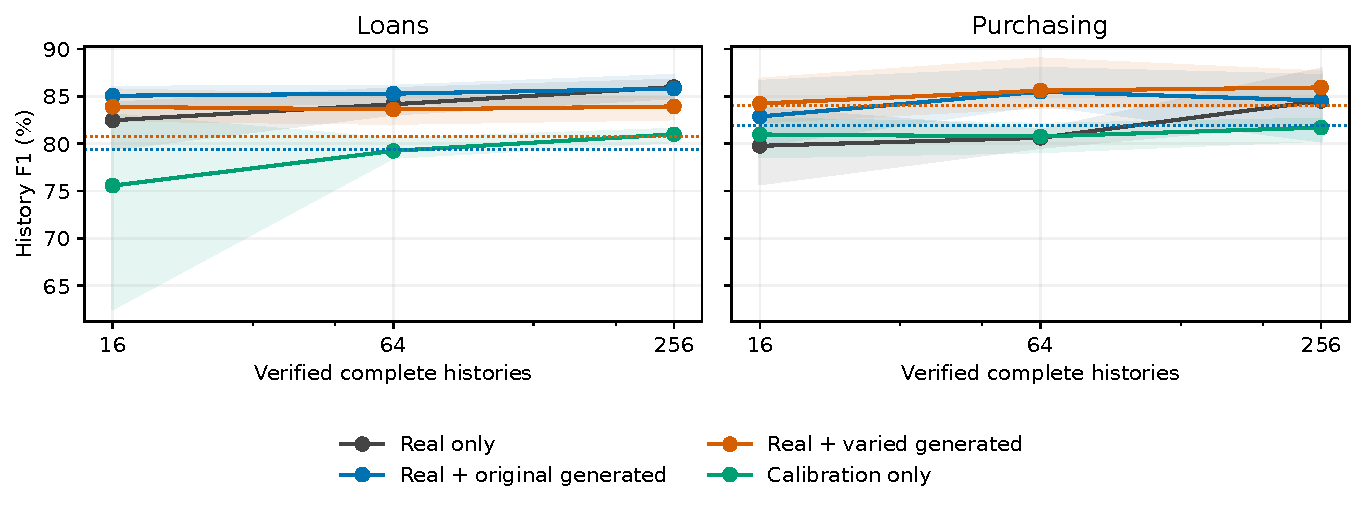
\includegraphics[width=\linewidth]{figures/budget_curves.pdf}
\caption{History recovery against complete verified-history budget. Lines show three-seed means; bands show observed minima and maxima, not confidence intervals. Dotted lines show fixed generated scorers without new target verification.}
\label{fig:budget-curves}
\end{figure}
